% Copyright (C) 2010,2011,2012,2013,2014,2015,2016 The ESPResSo project
% Copyright (C) 2002,2003,2004,2005,2006,2007,2008,2009,2010 
%  Max-Planck-Institute for Polymer Research, Theory Group
%  
% This file is part of ESPResSo.
%   
% ESPResSo is free software: you can redistribute it and/or modify it
% under the terms of the GNU General Public License as published by the
% Free Software Foundation, either version 3 of the License, or (at your
% option) any later version.
%  
% ESPResSo is distributed in the hope that it will be useful, but
% WITHOUT ANY WARRANTY; without even the implied warranty of
% MERCHANTABILITY or FITNESS FOR A PARTICULAR PURPOSE.  See the GNU
% General Public License for more details.
%  
% You should have received a copy of the GNU General Public License
% along with this program.  If not, see <http://www.gnu.org/licenses/>.
%
\chapter{First steps}
\label{chap:firststeps}

\section{Quick installation}

\index{configure}\index{make}

If you have installed the requirements (see section
\vref{sec:requirements}) in standard locations, to compile \es{}, it
is usually enough to execute the following sequence of two steps in
the directory where you have unpacked the sources:
\begin{code}
./configure
make
\end{code}

This will compile \es in a freshly created object path named according
to your CPU and operating system. As you have not yet specified a
configuration, a standard version will be built with the most often
used features. Usually you will want to build another version of \es
with options better suited for your purpose.

In some cases, \eg when \es needs to be compiled for several different
platforms or when different versions with different sets of features
are required, it might be useful to execute the commands not in the
source directory itself, but to start \texttt{configure} from another
directory (see section \vref{ssec:builddir}). Furthermore, many
features of \es can be selectively turned on or off in the local
configuration header (see section \vref{sec:myconfig}) before starting
the compilation with \texttt{make}.

The shell script \texttt{configure} prepares the source code for
compilation. It will determine how to use and where to find the
different libraries and tools required by the compilation process, and
it will test what compiler flags are to be used.  The script will find
out most of these things automatically.  If something is missing, it
will complain and give hints on how to solve the problem.  The
configuration process can be controlled with the help of a number of
options that are explained in section \vref{sec:configure}.

The command \texttt{make} will compile the source code. Depending on
the options passed to the program, \texttt{make} can also be used for
a number of other things:
\begin{itemize}
\item It can install and uninstall the program to some other
  directories. However, normally it is not necessary to actually
  \textit{install} \es to run it.
\item It can test \es for correctness.
\item It can build the documentation.
\end{itemize}
The details of the usage of \texttt{make} are described in section
\vref{sec:make}.

When these steps have successfully completed, \es can be started
with the command (see section \vref{sec:run})
\begin{code}
Espresso \var{script}
\end{code}
where \var{script} is a Tcl script that tells \es what to do, and
has to be written by the user. You can find some examples in the
\texttt{samples} folder of the source code directory.
If you want to run in parallel, you should have compiled \es to use
MPI, and need to tell MPI to run \es in parallel. The actual
invocation is implementation dependent, but in many cases, such as
OpenMPI, you can use
\begin{code}
mpirun -n \var{n\_nodes} Espresso \var{script}
\end{code}
where \var{n\_nodes} is the number of prcessors to be used.


\section{Running \es}

\subsection{Python}
\es is implemented as a Python module.
This means that you need to write a python script for any task you want to
perform with \es. In this chapter, the basic structure of the interface will be explained. For a practical introduction, see the tutorials, which are also part of the \es distribution.
To use \es, you need to import the espressomd module in your Python script. To this end, the folder containing the python module needs to be in the Python search path. The module is located in the src/python folder under the build directory.
A convenient way to run python with the correct path is to use the pypresso script located in the build directory. 
\begin{verbatim}
pypresso simulation.py
\end{verbatim}



\subsection{Tcl (deprecated)}
\es is implemented as an extension to the Tcl scripting language.
This means that you need to write a script for any task you want to
perform with \es. To learn about the Tcl script language and
especially the \es extensions, this chapter offers two tutorial
scripts. The first will guide you step-by-step through creating your
first simulation script, while the second script is a well documented
example simulation script. Since the latter is slightly more complex
and uses more advanced features of \es, we recommend to work through
both scripts in the presented order.  If you want to learn about the
Tcl language in greater detail, there is an excellent tutorial
\footnote{\url{http://www.tcl.tk/man/tcl8.5/tutorial/tcltutorial.html}}.


\section{Python: Basic concepts}
In this section, a brief overview is given over the most important components of the Python interface and their usage is illustrated by short examples.
The interface is contained in the espressomd Python module, which needs to be imported, before anything \es related can be done.
\begin{lstlisting}[language=python]
import espressomd
\end{lstlisting}
Access to the simulation system is provided via the System class. As a first step, an instance of the class needs to be created
\begin{lstlisting}[language=python]
system=espressomd.System()
\end{lstlisting}
Note that only one instance of the System class can be created, due to limitations in the simulation core.
Properties of the System class are used to access the parameters concerning the simulation system as a whole, \eg, the box geometry and the time step
\begin{lstlisting}[language=python]
system.box_l =(10.0,10.0,15.0)
print system.time_step
\end{lstlisting}


The particles in the simulation are accessed via the ParticleList class. It is used to retrieve individual particles of the simulation as well as for adding particles.
An instance of the class is provided as the part attribute of the System class.
Individual particles can be retrieved by their numerical id by using angular brackets
\begin{lstlisting}[language=python]
p=system.part[0]
\end{lstlisting}
It is also possible to loop over all particles
\begin{lstlisting}[language=python]
for p in system.part:
    ...
\end{lstlisting}
Particles are added via the add method
\begin{lstlisting}[language=python]
p=system.part.add(id=1,pos=(3.0,0.5,1.0),q=1)
\end{lstlisting}
An individual particle is represented by an instance of ParticleHandle.
The properties of the particle are implemented as Python properties:
\begin{lstlisting}[language=python]
p=system.part[0]
p.pos=(0,0,0)
print p.id,p.pos
system.part[0].q=-1
\end{lstlisting}
Properties of several particles can be accessed by using Python ranges
\begin{lstlisting}[language=python]
v=system.part[:].v
\end{lstlisting}

Interactions between particles fall in three categories:
\begin{itemize}
\item Non-bonded interactions are short-ranged interactions between \emph{all} pairs of particles of specified types. An example is the Lennard-Jones interaction mimicking overlap repulsion and van der Wals attraction. 
\item Bonded interactions act only between two specific particles. An example is the harmonic bond between adjacent particles in a polymer chain.
\item Long-range interactions act between all particles with specific properties in the entire system. An example is the coulomb interaction.
\end{itemize}

Non-bonded interactions are represented as subclasses of NonBondedInteraction, \eg LennardJonesInteraction. Instances of these classes for a given pair of particle types are accessed via the non_bonded_inter attribute of the System class. Parameters are set as follows
\begin{lstlisting}[language=python]
system.non_bonded_inter[0,0].lennard_jones.set_params(epsilon=1,sigma=1,cutoff=1.5,shift="auto")
\end{lstlisting}


Bonded interactions are represented by subclasses of BondedInteraction. To set up a bonded interaction, first an instance of the appropriate class is created with the desired parameters. Then, the bonded interaction is registered with the simulation core. Finally, the bond can be added to particles using the add_bond()-method of ParticleHandle with the instance of the bond class and the id of the bond partner particle. 
\begin{lstlisting}[language=python]
from interactions import HarmonicBond
harmonic=HarmonicBond(k=1,r_0=1)
system.bonded_inter.add(harmonic)
system.part[0].add_bond((harmonic,1))
system.part[1].add_bond((harmonic,2))
\end{lstlisting}

Long-range interactions are subclasses of Actor. They are used by first creating an instance of the desired actor and then adding it to the system.
To activate the P3M electrostatics solver, execute
\begin{lstlisting}[language=python]
from electrostatics import P3M
p3m=P3M(accuracy=1E-3, bjerrum_length=1)
system.actors.add(p3m)
\end{lstlisting}

\todo{Integrator, once the interface for that is clear}

\section{Tcl: Creating the first simulation script}

This section introduces some of the features of \es by constructing
step by step a simulation script for a simple salt crystal.  We cannot
give a full Tcl tutorial here; however, most of the constructs should
be self--explanatory. We also assume that the reader is familiar with
the basic concepts of a MD simulation here. The code pieces can be
copied step by step into a file, which then can be run using
\codebox{Espresso \textit{file}} from the \es source directory.

Our script starts with setting up the initial configuration.  Most
conveniently, one would like to specify the density and the number of
particles of the system as parameters:
\begin{tclcode}
set n_part 200; set density 0.7
set box_l [expr pow($n_part/$density,1./3.)]
\end{tclcode}
These variables do not change anything in the simulation engine, but
are just standard Tcl variables; they are used to increase the
readability and flexibility of the script. The box length is not a
parameter of this simulation; it is calculated from the number of
particles and the system density. This allows to change the parameters
later easily, \eg to simulate a bigger system.

The parameters of the simulation engine are modified by the
\verb|setmd| command. For example
\begin{tclcode}
setmd box_l $box_l $box_l $box_l
setmd periodic 1 1 1
\end{tclcode}
defines a cubic simulation box of size \verb|box_l|, and periodic
boundary conditions in all spatial dimensions. We now fill this
simulation box with particles
\begin{tclcode}
set q 1; set type 0
for {set i 0} { $i < $n_part } {incr i} {
  set posx [expr $box_l*[t_random]]
  set posy [expr $box_l*[t_random]]
  set posz [expr $box_l*[t_random]]
  set q [expr -$q]; set type [expr 1-$type]
  part $i pos $posx $posy $posz q $q type $type 
}
\end{tclcode}
This loop adds \verb|n_part| particles at random positions, one by
one.  In this construct, only two commands are not standard Tcl
commands: the random number generator \verb|t_random| and the
\verb|part| command, which is used to specify particle properties,
here the position, the charge \verb|q| and the type. In \es\ the
particle type is just an integer number which allows to group
particles; it does not imply any physical parameters. Here we use it
to tag the charges: positive charges have type 0, negative charges
have type 1.

Now we define the ensemble that we will be simulating. This is done
using the \verb|thermostat| command. We also set some integration
scheme parameters:
\begin{tclcode}
setmd time_step 0.01; setmd skin 0.4
set temp 1; set gamma 1
thermostat langevin $temp $gamma
\end{tclcode}
This switches on the Langevin thermostat for the NVT ensemble, with
temperature \verb|temp| and friction \verb|gamma|. The skin depth
\verb|skin| is a parameter for the link--cell system which tunes its
performance, but cannot be discussed here.

Before we can really start the simulation, we have to specify the
interactions between our particles.  We use a simple, purely repulsive
Lennard-Jones interaction to model the hard core repulsion
\citep{grest86a}, and the charges interact via the Coulomb potential:
\begin{tclcode}
set sig 1.0; set cut   [expr 1.12246*$sig]
set eps 1.0; set shift [expr 0.25*$eps]
inter 0 0 lennard-jones $eps $sig $cut $shift 0
inter 1 0 lennard-jones $eps $sig $cut $shift 0
inter 1 1 lennard-jones $eps $sig $cut $shift 0
inter coulomb 10.0 p3m tunev2 accuracy 1e-3 mesh 32
\end{tclcode}
The first three \verb|inter| commands instruct \es\ to use the same
purely repulsive Lennard--Jones potential for the interaction between
all combinations of the two particle types 0 and 1; by using different
parameters for different combinations, one could simulate differently
sized particles.  The last line sets the Bjerrum length to the value
10, and then instructs \es\ to use P$^3$M for the Coulombic
interaction and to try to find suitable parameters for an rms force
error below $10^{-3}$, with a fixed mesh size of 32. The mesh is fixed
here to speed up the tuning; for a real simulation, one will also tune
this parameter.

If we want to calculate the temperature of our system from the kinetic
energy, we need to know the number of the degrees of freedom of the
particles.  In \es these are usually 3 translational plus 3 rotational
degrees of freedom (if the feature ROTATION is activated). You can get
this number in the following way \footnote{There also exists a Tcl
  function \codebox{degrees_of_freedom} which does the same.}:

\begin{tclcode}
   if { [regexp "ROTATION" [code_info]] } { 
     set deg_free 6
   } else { set deg_free 3 }
\end{tclcode}

Now we can integrate the system:
\begin{tclcode}
set integ_steps 200
for {set i 0} { $i < 20 } { incr i} {
  set temp [expr [analyze energy kinetic]/(($deg_free/2.0)*$n_part)]
  puts "t=[setmd time] E=[analyze energy total], T=$temp"
  integrate $integ_steps 
}
\end{tclcode}
This code block is the primary simulation loop and runs
$20\times$\verb|integ_steps| MD steps. Every \verb|integ_steps| time steps, the
potential, electrostatic and kinetic energies are printed out (the latter one as
temperature). However, the simulation will crash: \es\ complains about particle
coordinates being out of range. The reason for this is simple: Due to the
initial random setup, the overlap energy is around a million kT, which we first
have to remove from the system. In \es, this is can be accelerated by capping
the forces, i.~e.\ modifying the Lennard--Jones force such that it is constant
below a certain distance. Before the integration loop, we therefore insert this
equilibration loop:
\begin{tclcode}
for {set cap 20} {$cap < 200} {incr cap 20} {
  puts "t=[setmd time] E=[analyze energy total]"
  inter forcecap $cap; integrate $integ_steps 
}
inter forcecap 0
\end{tclcode}
This loop integrates the system with a force cap of initially 20 and finally
200.  The last command switches the force cap off again. With this
equilibration, the simulation script runs fine.

However, it takes some time to simulate the system, and one will probably like
to write out simulation data to configuration files, for later analysis. For
this purpose \es\ has commands to write simulation data to a Tcl stream
in an easily parsable form.  We add the following lines at end of integration
loop to write the configuration files ``config\_0'' through ``config\_19'':
\begin{tclcode}
set f [open "config_$i" "w"]
blockfile $f write tclvariable {box_l density}
blockfile $f write variable box_l
blockfile $f write particles {id pos type}
close $f
\end{tclcode}
The created files ``config\_...'' are human--readable and look like
\begin{tclcode}
{tclvariable
        {box_l 10}
        {density 0.7}
}
{variable  {box_l 10.0 10.0 10.0} }
{particles {id pos type}
        {0 3.51770181433 4.3208975936 5.30529948918 0}
        {1 3.93145531704 6.58506447035 6.95045147034 1}
        ...
}
\end{tclcode}
As you can see, such a \emph{blockfile} consists of several Tcl lists,
which are called \emph{blocks}, and can store any data available from the
simulation. Reading a configuration is done by the following simple script:
\begin{tclcode}
set f [open $filename "r"]
while { [blockfile $f read auto] != "eof" } {}
close $f
\end{tclcode}
The \verb|blockfile read auto| commands will set the Tcl variables \verb|box_l|
and \verb|density| to the values specified in the file when encountering the
\verb|tclvariable| block, and set the box dimensions for the simulation when
encountering the \verb|variable| block. The particle positions and types of all
216 particles are restored when the \verb|particles| block is read. Note that it
is important to have the box dimensions set before reading the particles, to
avoid problems with the periodic boundary conditions.

\begin{figure}[tb]
  \centering
  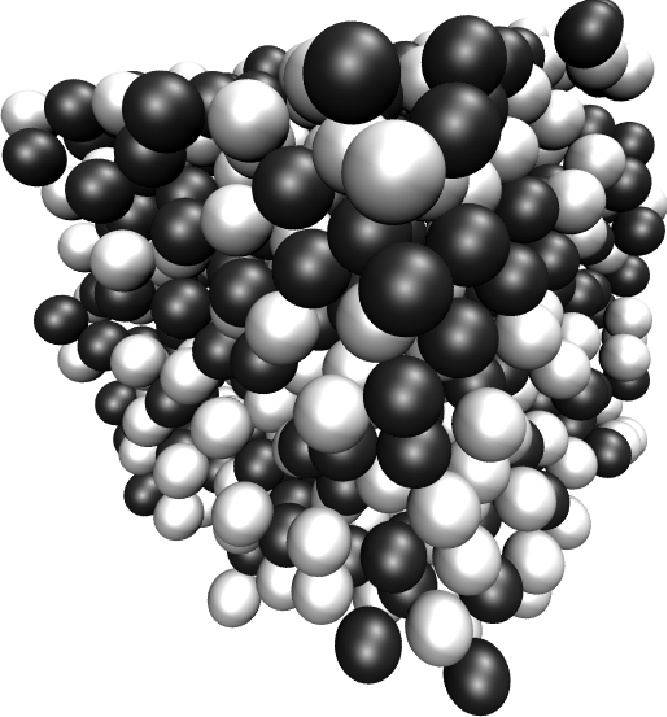
\includegraphics[width=0.4\textwidth]{figures/salt.png}
  \caption{VMD Snapshot of the salt system}
  \label{fig:snapshot}
\end{figure}

With these configurations, we can now investigate the system. As an example, we
will create a second script which calculates the averaged radial distribution
functions $g_{++}(r)$ and $g_{+-}(r)$. The radial distribution function for a
the current configuration can be obtained using the \verb|analyze| command:
\begin{tclcode}
set rdf [analyze rdf 0 1 0.9 [expr $box_l/2] 100]
set rlist ""
set rdflist ""
foreach value [lindex $rdf 1] {
  lappend rlist   [lindex $value 0]
  lappend rdflist [lindex $value 1] 
}
\end{tclcode}
The shown \verb|analyze rdf| command returns the distribution function of
particles of type 1 around particles of type 0 (i.~e.\ of opposite charges) for
radii between $0.9$ and half the box length, subdivided into $100$ bins.
Changing the first two parameters to either ``0 0'' or ``1 1'' allows to
determine the distribution for equal charges. The result is a list of $r$ and
$g(r)$ pairs, which the following foreach loop divides up onto two lists
\verb|rlist| and \verb|rdflist|.

To average over a set of configurations, we put the two last code snippets into
a loop like this:
\begin{tclcode}
set cnt 0
for {set i 0} {$i < 100} {incr i} { lappend avg_rdf 0}
foreach filename $argv {
  set f [open $filename "r"]
  while { [blockfile $f read auto] != "eof" } {}
  close $f
  set rdf [analyze rdf 0 1 0.9 [expr $box_l/2] 100]
  set rlist ""
  set rdflist ""
  foreach value [lindex $rdf 1] {
     lappend rlist   [lindex $value 0]
     lappend rdflist [lindex $value 1] }
  set avg_rdf [vecadd $avg_rdf $rdflist]
  incr cnt 
}
set avg_rdf [vecscale [expr 1.0/$cnt] $avg_rdf]
\end{tclcode}
Initially, the sum of all $g(r)$, which is stored in \verb|avg_rdf|, is set to
0.  Then the loops over all configurations given by \verb|argv|, calculates
$g(r)$ for each configuration and adds up all the $g(r)$ in \verb|avg_rdf|.
Finally, this sum is normalized by dividing by the number of
configurations. Note the ``1.0/\$cnt''; this is necessary, since ``1/\$cnt'' is
interpreted as an integer division, which results in 0 for $\text{cnt}>1$.
\verb|argv| is a predefined variable: it contains all the command line
parameters. Therefore this script should be called like
\begin{code}
Espresso \var{script} [\var{config}... ]
\end{code}


\begin{figure}[tb]
  \centering
  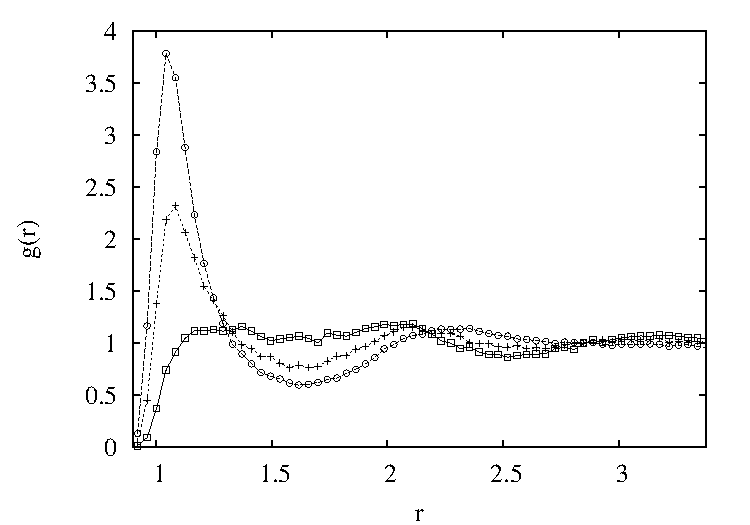
\includegraphics[width=0.7\textwidth]{figures/nacl-rdf.pdf}
  \caption{Radial distribution functions $g_{++}(r)$ between equal charges
    (rectangles) and $g_{+-}(r)$ for opposite charges (circles). The plus
    symbols denote $g(r)$ for an uncharged system.}
  \label{fig:rdf}
\end{figure}

The printing of the calculated radial distribution functions is simple. Add to the end of the
previous snippet the following lines:
\begin{tclcode}
set plot [open "rdf.data" "w"]
puts $plot "\# r rdf(r)"
foreach r $rlist rdf $avg_rdf { puts $plot "$r $rdf" }
close $plot
\end{tclcode}
This instructs the Tcl interpreter to write the \verb|avg_rdf| to the file \verb|rdf.data| in
gnuplot--compatible format. Fig.~\ref{fig:rdf} shows the resulting radial distribution functions,
averaged over 100 configurations. In addition, the distribution for a neutral
system is given, which can be obtained from our simulation script by simply
removing the command \verb|inter coulomb ...| and therefore not turning on P$^3$M.

The code example given before is still quite simple, and the reader is
encouraged to try to extend the example a little bit, e.~g. by using differently
sized particle, or changing the interactions. If something does not work, \es\
will give comprehensive error messages, which should make it easy to identify
mistakes. For real simulations, the simulation scripts can extend over thousands
of lines of code and contain automated adaption of parameters or online
analysis, up to automatic generation of data plots.  Parameters can be changed
arbitrarily during the simulation process, as needed for e.~g.\ simulated
annealing. The possibility to perform non--standard simulations without the need
of modifications to the simulation core was one of the main reasons why we
decided to use a script language for controlling the simulation core.

\section{Tcl: \texttt{tutorial.tcl}}

In the directory \texttt{samples/} of the es{} sources, you will find
a well documented simulation script \texttt{tutorial.tcl}, which takes
you step by step through a slightly more complicated simulation of a
polyelectrolyte system. The basic structure of the script is however
the same as in the previous example and probably the same as the
structure of most \es{} simulation scripts.

Initially, some parameters and global variables are set, the
interactions are initialized, and particles are added. For this, the
script makes use of the \verb|polymer| command, which provides a
faster way to set up chain molecules.

The actual simulation falls apart again into two loops, the warmup
loop with increasing force capping, and the final simulation loop.
Note that the electrostatic interaction is only activated after
equilibrating the excluded volume interactions, which speeds up the
warmup phase. However, depending on the problem, this splitted warmup
may not be possible due to physical restrictions. \es{} cannot detect
these mistakes and it is your responsibility to find simulation
procedure suitable to your specific problem.

%%% Local Variables: 
%%% mode: latex
%%% TeX-master: "ug"
%%% End: 
